\documentclass[a4paper,12pt]{article}

\usepackage[utf8]{inputenc}
\usepackage{geometry}
\usepackage{graphicx}
\usepackage{amsmath}
\usepackage{hyperref}

\geometry{margin=1in}

\title{Electronics Experiment Report:}
\author{B13901165張勝勛, B13901020陳諺德}
\date{\today}

% Language and font packages
\usepackage{ctex} % Chinese support

% Pseudocode and algorithm packages
% \usepackage{algorithm2e} % Advanced algorithm writing
% \usepackage{algpseudocode} % Pseudocode environment for algorithms

% Fancy style packages
\usepackage{fancyhdr} % Custom headers/footers
\usepackage{color} % Color support
\usepackage{xcolor} % Extended color support
\usepackage{tcolorbox} % Colored boxes
\usepackage{framed} % Framed environments

% Math and symbol packages
\usepackage{amsfonts}
\usepackage{amssymb}
\usepackage{mathtools}

% Table and figure packages
% \usepackage{booktabs} % Professional tables
% \usepackage{multirow} % Multi-row tables
% \usepackage{caption} % Custom captions
\usepackage{subcaption} % Subfigures

% Miscellaneous
\usepackage{enumitem} % Custom lists
\usepackage{listings} % Code listings
\usepackage{tikz} % Drawing diagrams
\usepackage{pgfplots} % For plotting graphs
\usepackage{float}

\begin{document}
\renewcommand{\figurename}{圖}
\maketitle

\section{Experiment setup}
\begin{figure}[H]
    \centering
    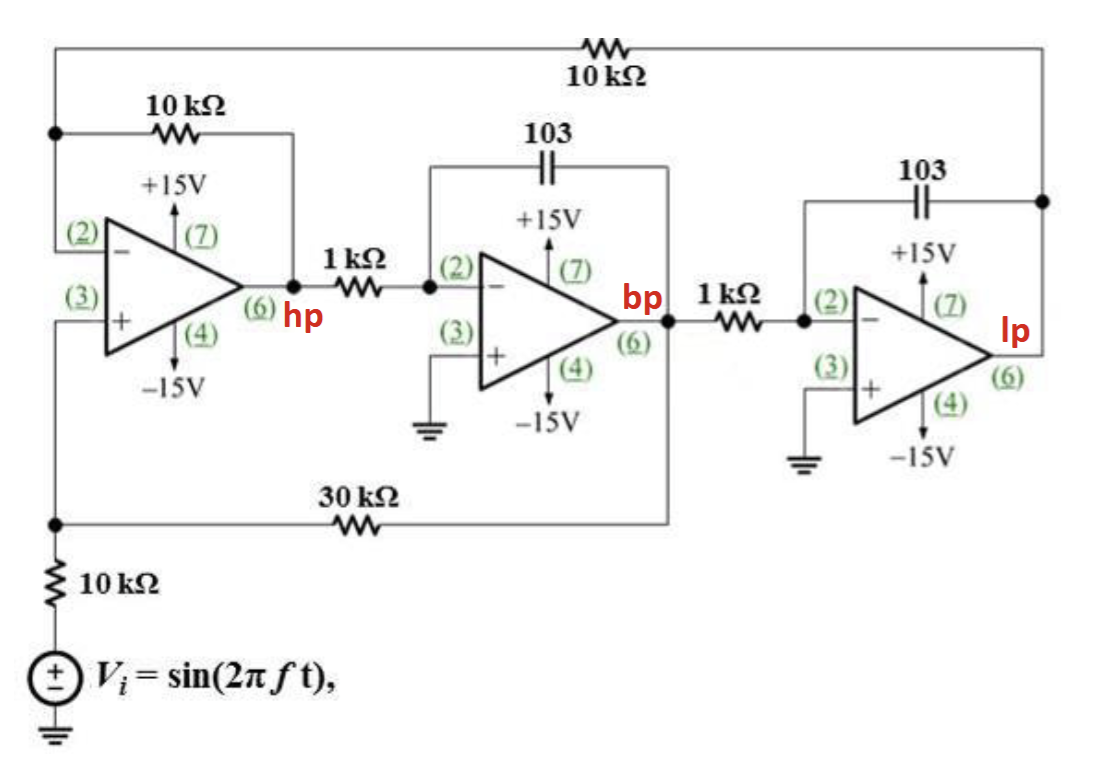
\includegraphics[width=0.8\textwidth]{exp_setup.png}
    \caption{Experiment setup}
    \label{fig:example}
\end{figure}

\section{Experiment results}
\subsection{original data table}
Here is the original data we collected from the experiment:
\begin{table}[H]
\centering
\begin{tabular}{|c|c|c|c|c|c|c|}
\hline
$f$ (kHz) & CH1 & CH2 & CH2/CH1 & $20\log(\text{CH2/CH1})$ & $\log(f)$ & 備註 \\ \hline
1.0 & 432 & 64 & 0.1481 & -16.5861 & 0.0000 &  \\
3.0 & 432 & 184 & 0.4259 & -7.4133 & 0.4771 &  \\
5.0 & 432 & 280 & 0.6481 & -3.7665 & 0.6990 &  \\
7.0 & 432 & 420 & 0.9722 & -0.2447 & 0.8451 &  \\
10.0 & 432 & 736 & 1.7037 & 4.6279 & 1.0000 &  \\
11.0 & 432 & 912 & 2.1111 & 6.4902 & 1.0414 & f3dB low \\
12.0 & 432 & 1090 & 2.5231 & 8.0389 & 1.0792 &  \\
15.0 & 432 & 1280 & 2.9630 & 9.4345 & 1.1761 &  \\
17.0 & 432 & 1060 & 2.4537 & 7.7964 & 1.2304 &  \\
18.0 & 432 & 960 & 2.2222 & 6.9357 & 1.2553 &  \\
18.5 & 432 & 904 & 2.0926 & 6.4137 & 1.2672 & f3dB high \\
19.0 & 432 & 856 & 1.9815 & 5.9398 & 1.2788 & \\
20.0 & 432 & 768 & 1.7778 & 4.9975 & 1.3010 & \\
30.0 & 432 & 400 & 0.9259 & -0.6685 & 1.4771 &  \\
50.0 & 432 & 232 & 0.5370 & -5.3999 & 1.6990 &  \\
100.0 & 432 & 144 & 0.3333 & -9.5424 & 2.0000 &  \\
200.0 & 432 & 128 & 0.2963 & -10.5655 & 2.3010 &  \\
\hline
\end{tabular}
\caption{frequency response data}
\label{tab:frequency_response}
\end{table}
\subsection{Bode plot}
Here is the Bode plot of the frequency response:
\begin{figure}[H]
    \centering
    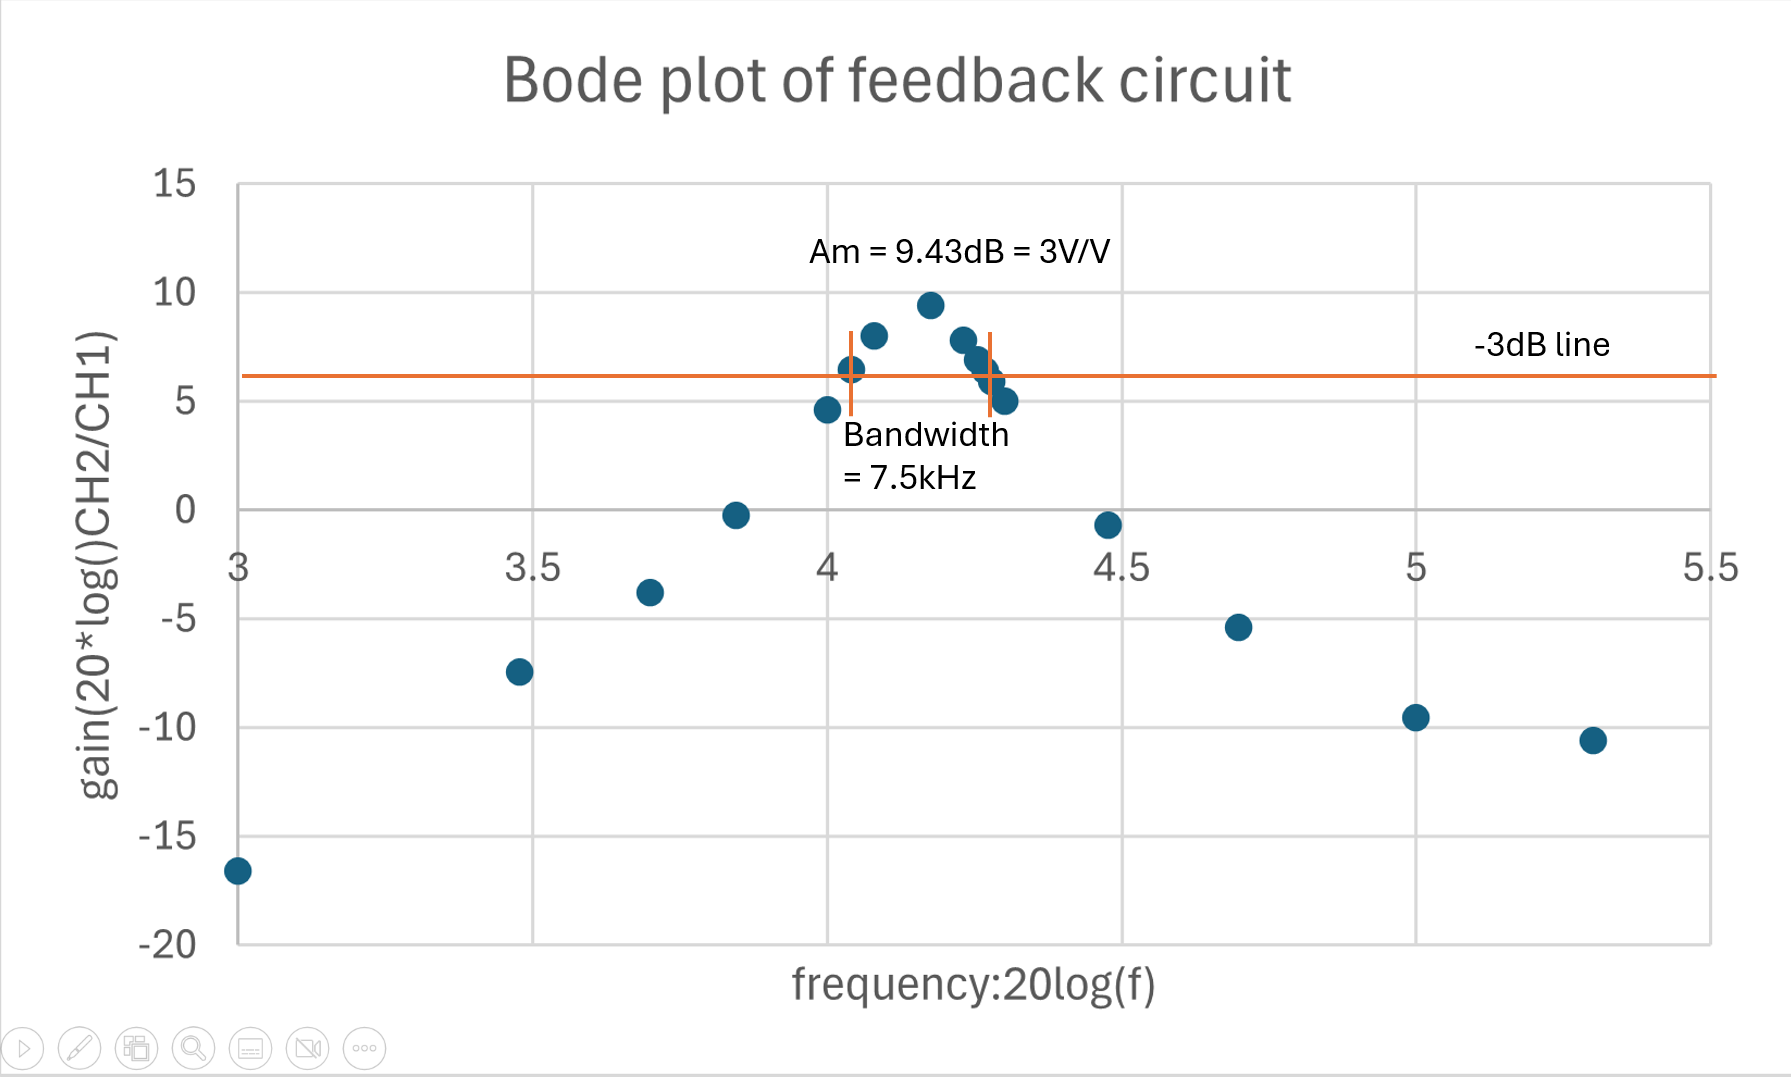
\includegraphics[width=0.8\textwidth]{bode_plot.png}
    \caption{Bode plot of the frequency response}
    \label{fig:bode_plot}
\end{figure}

\subsection{specific configuration}
The specific configuration of the circuit is as follows:
\begin{itemize}
    \item $f_{3dB,low} = 11.0$ kHz
    \item $f_{3dB,high} = 18.5$ kHz
    \item $BW = f_{3dB,high} - f_{3dB,low} = 7.5$ kHz
    \item $A_{max} = 2.96$ at $f = 15.0$ kHz
\end{itemize}

\section{reflection}
\begin{itemize}
    \item 陳諺德: In this experiment, I learned that we can get a band-pass, high-pass, and low pass filter by using three amp concatenated together.
Also, I learned more about the configuration of ua741 
    \item 張勝勛: Since the circuit configuration is more complicated this time, I learned how to choose the right length of wires to connect the circuit.
In this way, we can easily debug and reduce the possibility of short circuit.
\end{itemize}
\end{document}